\documentclass[12pt]{article}
\usepackage{fancyhdr}
\pagestyle{fancy}
\fancyhf{}
\fancyfoot[C]{\thepage}
\fancyfoot[L]{\scriptsize CC BY-NC-SA 4.0 \textbullet\ Leo Liang}
\renewcommand{\headrulewidth}{0pt}
\usepackage[margin=1in]{geometry}
\usepackage{amsmath, amssymb}
\usepackage{array, booktabs}
\usepackage{pgffor}
\usepackage{tikz}
\parindent=0pt
\parskip=1em
\newcolumntype{C}[1]{>{\centering\arraybackslash}p{#1}}
\newcommand{\wl}{\par\vspace{5mm}\noindent\rule{\linewidth}{0.4pt}\par\vspace{1mm}}
\newcommand{\wls}[1]{\foreach \i in {1,...,#1}{\wl}}
% tikz helper: a labeled square coordinate grid from -#1 to #1 (use inside a tikzpicture)
\newcommand{\gridaxes}[1]{%
  \draw[step=1,gray!25,very thin] (-#1,-#1) grid (#1,#1);%
  \draw[thick,->] (-#1-0.4,0)--(#1+0.4,0) node[right]{$x$};%
  \draw[thick,->] (0,-#1-0.4)--(0,#1+0.4) node[above]{$y$};%
  \foreach \n in {-#1,...,#1}{\ifnum\n=0\else
      \draw (\n,0.08)--(\n,-0.08) node[below]{\scriptsize$\n$};
      \draw (0.08,\n)--(-0.08,\n) node[left]{\scriptsize$\n$};\fi}%
}
% ─────────────────────────────────────────────────────────────────────────────
\begin{document}
\pagestyle{fancy}
\begin{center}
  {\Large\bfseries Homework 4}\\[4pt]
  The Coordinate Plane, Lines, and Reading Graphs\\[6pt]
  Name:\;\underline{\hspace{6.5cm}}\quad
\end{center}
\hrule\bigskip

\section*{Instructions}
This homework is mostly \textbf{reading} --- it teaches you brand-new material. Read each section \textbf{slowly,
with a pen}, and answer its questions before moving on. Write your own questions and any ``wait, what?'' moments
in the margin in a different color. You may use the internet or AI as a \textbf{teacher} (ask it to
explain or to give you extra examples), but always try the questions yourself first.

% ===========================================================================
\section*{Reading 1 --- The Coordinate Plane}
The \textbf{coordinate plane} is built from two number lines that cross at a point called the \textbf{origin}. The
horizontal one is the \textbf{$x$-axis}; the vertical one is the \textbf{$y$-axis}.

Every point is named by an \textbf{ordered pair} $(x,y)$. The first number $x$ says how far \textbf{right}
(positive) or \textbf{left} (negative) of the origin; the second number $y$ says how far \textbf{up} (positive) or
\textbf{down} (negative). \emph{Order matters:} $(2,5)$ and $(5,2)$ are different points.

You have seen ordered pairs before: a point $(x,y)$ is just an \textbf{(input, output)} pair --- the same kind you
used to describe functions. The coordinate plane is simply where we \emph{draw} those pairs.

\textbf{Example.} To plot $(3,2)$: start at the origin, go \textbf{right $3$}, then \textbf{up $2$}.

\begin{center}
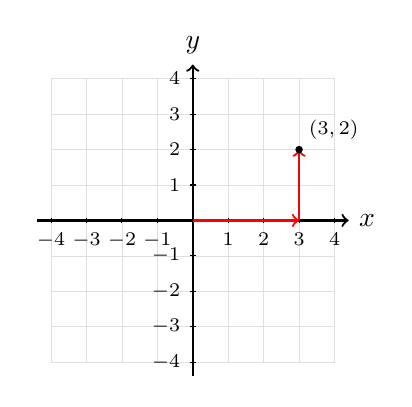
\begin{tikzpicture}[scale=0.45]
  \gridaxes{4}
  \draw[->,thick,red] (0,0)--(3,0);
  \draw[->,thick,red] (3,0)--(3,2);
  \fill (3,2) circle (3pt) node[above right]{\scriptsize$(3,2)$};
\end{tikzpicture}
\end{center}

The two axes split the plane into four \textbf{quadrants}, numbered I--IV counterclockwise starting from the
top-right.

\bigskip
\textbf{Q1.}\quad Plot and label these four points on the grid: $A=(3,2)$,\; $B=(-2,4)$,\; $C=(0,-3)$,\;
$D=(-4,-1)$.

\begin{center}
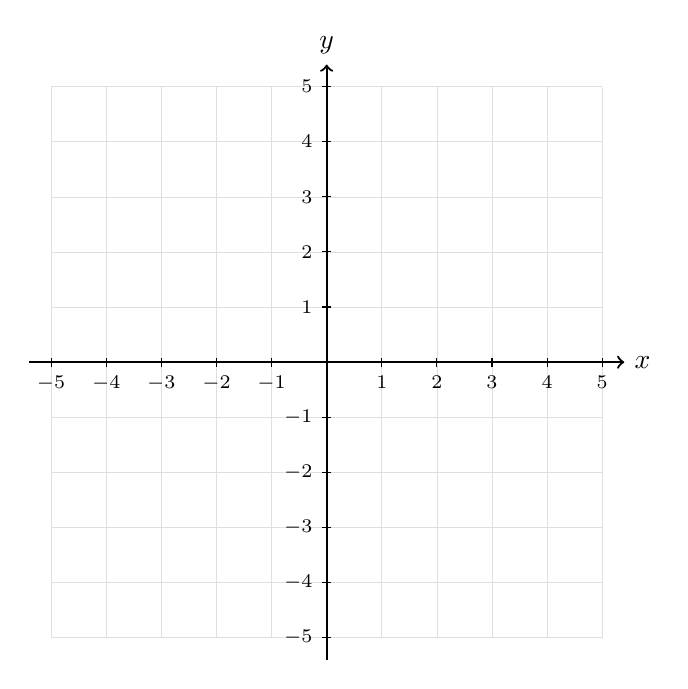
\begin{tikzpicture}[scale=0.7]
  \gridaxes{5}
\end{tikzpicture}
\end{center}

\textbf{Q2.}\quad Write the coordinates of each labeled point.

\begin{center}
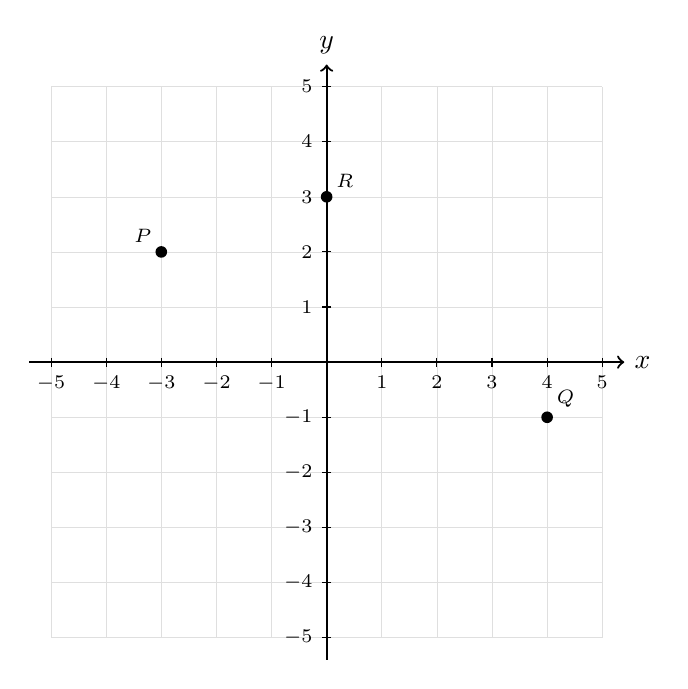
\begin{tikzpicture}[scale=0.7]
  \gridaxes{5}
  \fill (-3,2) circle (3pt) node[above left]{\scriptsize$P$};
  \fill (4,-1) circle (3pt) node[above right]{\scriptsize$Q$};
  \fill (0,3) circle (3pt) node[above right]{\scriptsize$R$};
\end{tikzpicture}
\end{center}
$P = \underline{\hspace{2.5cm}}$\qquad $Q = \underline{\hspace{2.5cm}}$\qquad $R = \underline{\hspace{2.5cm}}$

\medskip
\textbf{Q3.}\quad Answer in one sentence each. (a) The point $(4,0)$ sits on one of the axes --- which one?
(b) What is the special name for the point $(0,0)$? (c) Why are $(2,5)$ and $(5,2)$ different points?
\wls{6}

% ===========================================================================
\newpage
\section*{Reading 2 --- Graphing a Function}
A function takes an input $x$ and produces one output, written $y = f(x)$. To \textbf{graph} a function, we turn
each input--output pair into a point and plot it:
\[
  \text{input } x \;\longrightarrow\; \text{output } y = f(x) \;\longrightarrow\; \text{point } (x,\,f(x)).
\]
The \textbf{graph} of a function is the picture of \emph{all} of its $(x,\,f(x))$ points. (This is the ``graph''
representation of a function from our last unit.)

\textbf{How to graph one:} (1)~pick some inputs; (2)~compute their outputs in a table; (3)~plot the points;
(4)~connect them.

\textbf{A caution about connecting the dots.}\quad When we connect plotted points with straight segments, we are
quietly \emph{assuming} that the function really runs along those segments --- that the in-between values lie
exactly on our line. For a \textbf{linear} function (a straight line) this is true, so connecting the dots is
exact. But for any other function it is only an \textbf{estimate}: the real graph may curve above or below the
line between two points. To see the true shape of a non-linear function, you have to plot \emph{more} points and
look closely. (You will meet exactly such a curve in the Challenge.)

\textbf{Example.} For $f(x) = x+1$:

\medskip
\renewcommand{\arraystretch}{1.5}
\begin{tabular}{|C{1.5cm}|C{1.5cm}|C{1.5cm}|C{1.5cm}|C{1.5cm}|}
\hline
$x$ & $-2$ & $-1$ & $0$ & $1$ \\
\hline
$f(x)$ & $-1$ & $0$ & $1$ & $2$ \\
\hline
\end{tabular}
\renewcommand{\arraystretch}{1}

\medskip
Plotting these points and connecting them gives a straight line. You can try this for yourself.

\newpage
\bigskip
\textbf{Q4.}\quad Let $f(x) = 2x - 1$. Complete the table, then plot the points and connect them.

\medskip
\renewcommand{\arraystretch}{2}
\begin{tabular}{|C{2cm}|C{2cm}|C{2cm}|C{2cm}|C{2cm}|}
\hline
$x$ & $-2$ & $-1$ & $0$ & $1$ \\
\hline
$f(x)$ & & & & \\
\hline
\end{tabular}
\renewcommand{\arraystretch}{1}

\begin{center}
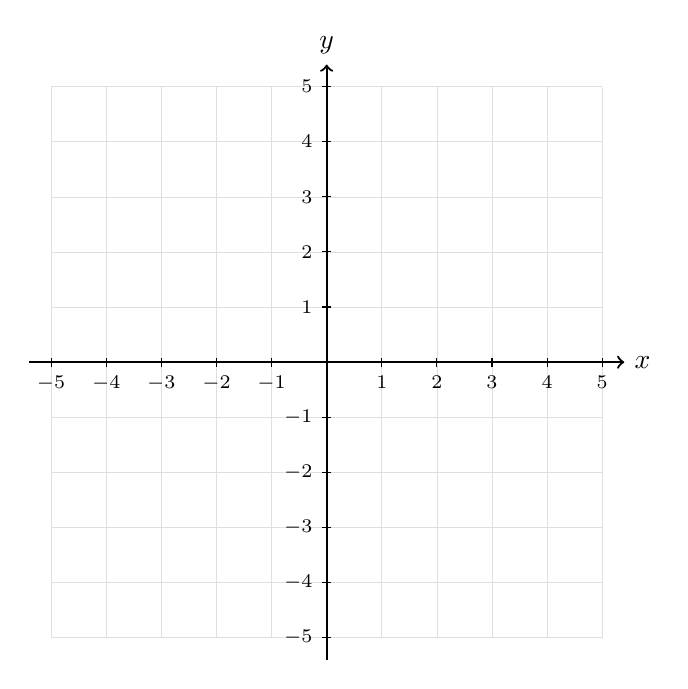
\begin{tikzpicture}[scale=0.7]
  \gridaxes{5}
\end{tikzpicture}
\end{center}

\textbf{Q5.}\quad Using the line you drew in Q4: (a) what is $f(3)$? \quad (b) for what $x$ is $f(x) = 5$?
\wls{4}

% ===========================================================================
\newpage
\section*{Reading 3 --- Lines and Slope (Rate of Change)}
Some functions graph as perfectly straight \textbf{lines} while others don't. The most important number for a line is its
\textbf{slope} --- how steep it is and which way it tilts.
\[
  \text{slope} = \frac{\text{rise}}{\text{run}} = \frac{\text{change in } y}{\text{change in } x}.
\]
In words: for every step you take to the \emph{right} (the run), how far \emph{up or down} does the line go (the
rise)? From two points $(x_1,y_1)$ and $(x_2,y_2)$,
\[
  m = \frac{y_2 - y_1}{x_2 - x_1}.
\]
A \textbf{positive} slope goes uphill (left to right); a \textbf{negative} slope goes downhill; a \textbf{zero}
slope is flat. A \textbf{vertical} line is special: its run is $0$, and you cannot divide by $0$, so its slope is
\textbf{undefined}.

The big idea for later: \textbf{slope is a rate of change} --- it measures how fast $y$ changes as $x$ changes.

\textbf{Example.} The line through $(0,1)$ and $(2,5)$: $\;m = \dfrac{5-1}{2-0} = \dfrac{4}{2} = 2$. That is,
``up $2$ for every $1$ to the right.''

\bigskip
\textbf{Q6.}\quad Find the slope of the line through $(1,2)$ and $(4,11)$. Show the rise and the run.
\wls{2}

\textbf{Q7.}\quad For each line, is the slope positive, negative, zero, or undefined?

\medskip
\textbf{(a)}\quad uphill from left to right \hfill \underline{\hspace{3cm}}

\medskip
\textbf{(b)}\quad flat and horizontal \hfill \underline{\hspace{3cm}}

\medskip
\textbf{(c)}\quad straight up and vertical \hfill \underline{\hspace{3cm}}

\medskip
\textbf{(d)}\quad downhill from left to right \hfill \underline{\hspace{3cm}}

\newpage
\medskip
\textbf{Q8.}\quad Find the slope of the line drawn below by reading its rise and run off the grid.

\begin{center}
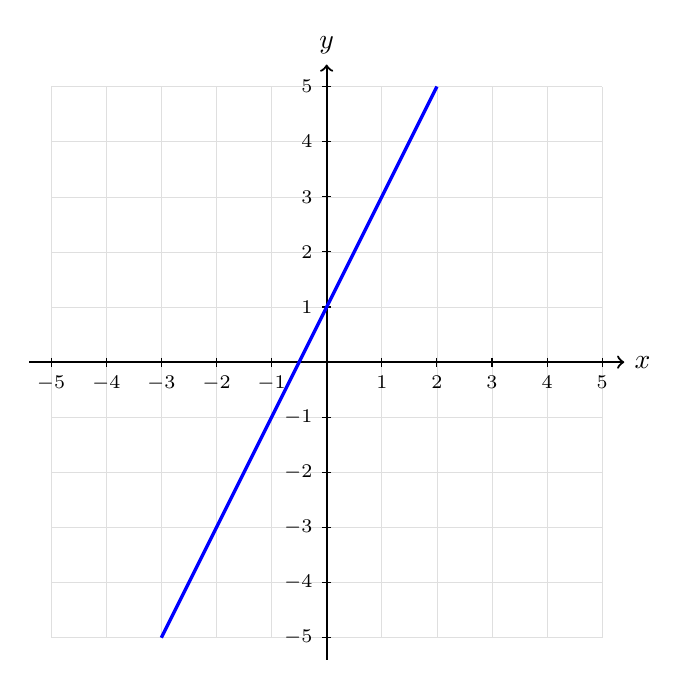
\begin{tikzpicture}[scale=0.7]
  \gridaxes{5}
  \draw[very thick,blue] (-3,-5)--(2,5);
\end{tikzpicture}
\end{center}
Slope $=\;\underline{\hspace{3cm}}$

%==================================================================

\newpage
\section*{Reading 4 --- What Makes a Function Linear?}
We keep using the word \textbf{linear} --- here is what it actually means.

A function is \textbf{linear} when its rate of change (its slope) is the \textbf{same everywhere}: no matter which
two points you pick, you get the \emph{same} slope. Because the steepness never changes, the graph is a perfectly
straight \textbf{line}. That single idea can be said three equivalent ways:
\begin{itemize}
  \item \textbf{As a picture:} the graph is a straight line.
  \item \textbf{As an equation:} it can be written $y = mx + b$ (a constant slope $m$ and a constant starting
        value $b$).
  \item \textbf{As a rate:} the rate of change is constant --- equal steps in $x$ always produce equal steps in
        $y$.
\end{itemize}

\textbf{A test you can run on any table.} Step $x$ up by the same amount each time and watch the outputs. If the
outputs change by the \emph{same} amount every step, the function is linear. If those jumps keep changing, it is
not.

\medskip
\textit{Linear} --- the steps in $y$ are constant:

\medskip
\renewcommand{\arraystretch}{1.5}
\begin{tabular}{|C{2.6cm}|C{1.2cm}|C{1.2cm}|C{1.2cm}|C{1.2cm}|}
\hline
$x$ & $0$ & $1$ & $2$ & $3$ \\
\hline
$f(x) = 2x-1$ & $-1$ & $1$ & $3$ & $5$ \\
\hline
\end{tabular}
\renewcommand{\arraystretch}{1}

Step changes in $f(x)$: $\;+2,\ +2,\ +2\;$ --- \textbf{constant}, so $f$ is \textbf{linear}.

\medskip
\textit{Not linear} --- the steps in $y$ keep growing:

\medskip
\renewcommand{\arraystretch}{1.5}
\begin{tabular}{|C{2.6cm}|C{1.2cm}|C{1.2cm}|C{1.2cm}|C{1.2cm}|}
\hline
$x$ & $0$ & $1$ & $2$ & $3$ \\
\hline
$g(x) = x^2$ & $0$ & $1$ & $4$ & $9$ \\
\hline
\end{tabular}
\renewcommand{\arraystretch}{1}

Step changes in $g(x)$: $\;+1,\ +3,\ +5\;$ --- \textbf{keeps growing}, so $g$ is \textbf{not} linear.

\medskip
\textbf{Non-linear functions.} When the rate of change \emph{keeps changing}, the graph bends --- it is a
\textbf{curve}, not a straight line. (Careful with words: a ``line'' is \emph{always} straight, so we do not say
``non-linear line'' --- we say \textbf{non-linear function}, and its graph is a curve.) The function $g(x)=x^2$ is
the classic example: in the Challenge you will see its average rate of change is $3$ between $x=1$ and $x=2$ but
$5$ between $x=2$ and $x=3$. The slope is different in different places, so the graph curves --- and handling that
changing rate is exactly what calculus is built for.

\bigskip
\textbf{Q.}\quad For each table, find the change in $y$ at each step, then say whether the function is
\textbf{linear} or \textbf{non-linear} and how you know.

\medskip
(a)\quad
\begin{tabular}{|C{1.1cm}|C{1.1cm}|C{1.1cm}|C{1.1cm}|}
\hline
$x$ & $0$ & $1$ & $2$ \\
\hline
$y$ & $4$ & $7$ & $10$ \\
\hline
\end{tabular}
\qquad
(b)\quad
\begin{tabular}{|C{1.1cm}|C{1.1cm}|C{1.1cm}|C{1.1cm}|}
\hline
$x$ & $0$ & $1$ & $2$ \\
\hline
$y$ & $1$ & $2$ & $5$ \\
\hline
\end{tabular}
\wls{4}

\textbf{Q.}\quad Which of these are linear? Circle them, and for each one that is not, say what makes it non-linear.
\[
  y = 3x + 2, \qquad y = x^2, \qquad y = -x, \qquad y = \tfrac{1}{x}.
\]
\wls{4}

% ===========================================================================
\newpage
\section*{Reading 5 --- The Equation of a Line: $y = mx + b$}
Every non-vertical line can be written in the form
\[
  y = mx + b,
\]
where $m$ is the \textbf{slope} and $b$ is the \textbf{$y$-intercept} --- the $y$-value where the line crosses the
$y$-axis (the output when $x = 0$, the ``starting value'').

\textbf{To graph from $y = mx + b$:} start at the point $(0,b)$ on the $y$-axis, then use the slope to step:
right $1$, up $m$ (down if $m$ is negative). Repeat to get more points, then draw the line.

\textbf{Example.} $y = 3x - 2$: the $y$-intercept is $b = -2$, so start at $(0,-2)$; the slope is $m = 3$, so go up
$3$ and right $1$.

\textbf{Reading $m$ and $b$ off a graph:} the slope $m$ is the rise over the run between any two points on the
line; the $y$-intercept $b$ is the height where the line crosses the $y$-axis.

\bigskip
\textbf{Q9.}\quad For $y = -2x + 4$:

\medskip
\textbf{(a)}\quad the slope is \hfill \underline{\hspace{3cm}}

\medskip
\textbf{(b)}\quad the $y$-intercept is \hfill \underline{\hspace{3cm}}

\medskip
\textbf{(c)}\quad Graph the line on the grid (start at the intercept, then use the slope).

\begin{center}
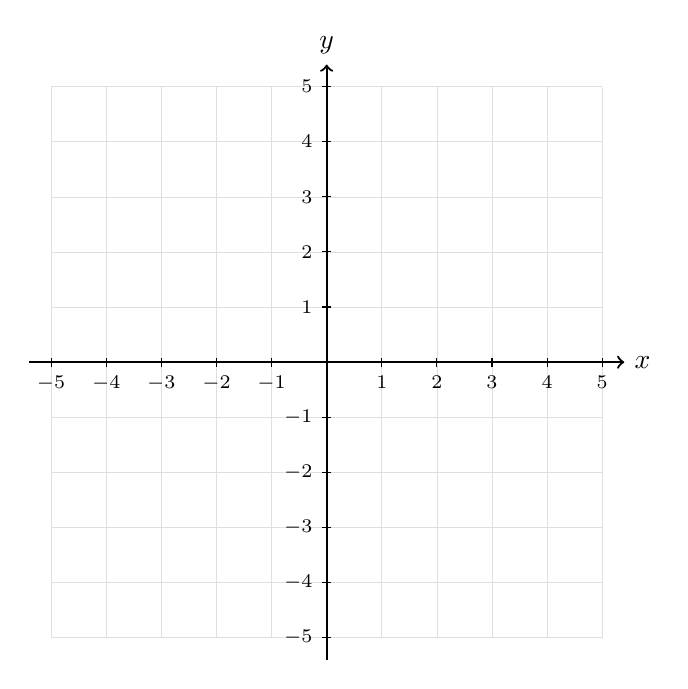
\begin{tikzpicture}[scale=0.7]
  \gridaxes{5}
\end{tikzpicture}
\end{center}

\textbf{Q10.}\quad Write the equation $y = mx + b$ of the line with slope $\tfrac{1}{2}$ and $y$-intercept $-3$.
\wl

\textbf{Q11.}\quad Read the slope and the $y$-intercept off the line below, then write its equation.

\begin{center}
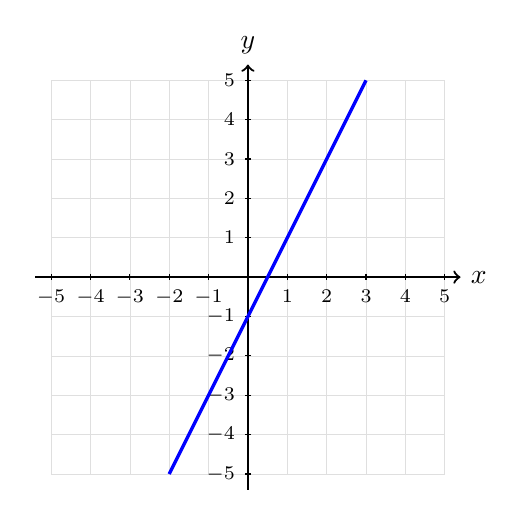
\begin{tikzpicture}[scale=0.5]
  \gridaxes{5}
  \draw[very thick,blue] (-2,-5)--(3,5);
\end{tikzpicture}
\end{center}
slope $=\;\underline{\hspace{2cm}}$\qquad $y$-intercept $=\;\underline{\hspace{2cm}}$\qquad
equation: $\;\underline{\hspace{4cm}}$

% ===========================================================================
\newpage
\section*{Reading 5 --- Reading Graphs in the Real World}
A graph tells a \textbf{story}. On a real-world line graph:
\begin{itemize}
  \item the \textbf{slope} is a \textbf{rate} --- how fast one quantity changes per unit of the other (miles per
        hour, dollars per item, blocks per minute);
  \item the \textbf{$y$-intercept} is a \textbf{starting amount} --- the value when the other quantity is $0$;
  \item a line going \textbf{up} means increasing, \textbf{down} means decreasing, and \textbf{flat} means not
        changing.
\end{itemize}
\textbf{Example.} If a graph shows distance (km) against time (hours), the slope is the \textbf{speed} (km per
hour), and the $y$-intercept is how far you had already travelled at time $0$.

\bigskip
\textbf{Q12.}\quad \textbf{Real-Life Application.} While mining, your total cobblestone $y$ (in blocks) after $x$
minutes follows $\;y = 5x + 10$.

\medskip
(a) What does the slope $5$ mean in this situation?
\wl
(b) What does the $10$ mean in this situation?
\wl
(c) How much cobblestone do you have after $6$ minutes?
\wl

\textbf{Q13.}\quad A graph of the water in a tank over time goes \textbf{uphill}, then \textbf{flat}, then
\textbf{downhill}. Describe in words what is happening to the water during each part, and what the slope is doing.
\wls{3}

% ===========================================================================
\newpage
\section*{Challenge --- When the Rate Keeps Changing}
A straight line has \emph{one} slope everywhere --- a single, constant rate. But many graphs are \textbf{curves},
and a curve's steepness \emph{changes} from point to point. We can still measure the \textbf{average rate of
change} between two points, using the very same rise-over-run idea.

Consider $f(x) = x^2$:

\medskip
\renewcommand{\arraystretch}{1.5}
\begin{tabular}{|C{1.5cm}|C{1.5cm}|C{1.5cm}|C{1.5cm}|C{1.5cm}|}
\hline
$x$ & $0$ & $1$ & $2$ & $3$ \\
\hline
$f(x)$ & $0$ & $1$ & $4$ & $9$ \\
\hline
\end{tabular}
\renewcommand{\arraystretch}{1}

\bigskip
\textbf{Q14.}\quad
(a) Find the average rate of change of $f$ between $x=1$ and $x=2$ (use $\frac{\text{change in } y}{\text{change
in } x}$).
\wl
(b) Find the average rate of change between $x=2$ and $x=3$.
\wl
(c) Are your two answers the same? What does that tell you about how the \emph{steepness} of this curve is
changing as you move to the right?
\wls{2}

\textit{(This question is the doorway to the next unit: when a rate keeps changing, how do we find the rate at a
single instant? That is where calculus begins.)}

% ===========================================================================
\newpage
\section*{Notebook Artifact (Metacognition)}

\textbf{N1.}\quad On the \textbf{left page} of your notebook, write \textbf{one Question-Compass} about
\emph{slope} (or about graphs), and \textbf{one muddiest point} --- the single idea from this homework you are
least sure about.

\bigskip
\textbf{N2.}\quad If you used the internet or AI, describe how you used it.
\wls{4}

\end{document}
